%%% All Your Base 2015
%%% http://allyourbaseconf.com/2015/speakers#dimitri-fontaine
%%% 
%%% PostgreSQL is YeSQL!
%%%
%%% The database landscape has changed a lot in the recent years. The NoSQL
%%% movement has taken the world by storm and you may wonder if there is
%%% still room for relational databases. In this talk we will learn about
%%% the strengths that make PostgreSQL more relevant than ever. We’ll survey
%%% its architecture, availability tradeoffs, durability with one or more
%%% servers, and yes even SQL!

%%% 
%%% WHAT WILL I LEARN?
%%% 
%%% From this talk you will learn to appreciate how versatile SQL really is
%%% and the many use-cases it can be applied to and solve elegantly. You
%%% will also be introduced to the basics for PostgreSQL High Availability
%%% and Scaling, a must-know in this time of high availability.

\documentclass{beamer}

\usepackage{tikz}
\usetikzlibrary{arrows,backgrounds,snakes,shadows}

\usepackage{minted}

\usepackage[utf8]{inputenc}

\usepackage{beamerthemesplit}
\usetheme{Boadilla}
%\setbeamertemplate{itemize items}{\checkmark}
\setbeamertemplate{itemize items}[circle]
\beamertemplatetransparentcovered

\usepackage{multicol}

\title{\textsc{PostgreSQL is YeSQL!}}
\subtitle{All Your Base Conference 2015}
\author{\textit{Dimitri Fontaine} \texttt{dimitri@2ndQuadrant.fr}
  \linebreak
  \url{@tapoueh}}
\date{13 November 2015}
\logo{
\includegraphics[height=0.4cm]{2ndQuadrant-cross.png}}

\begin{document}

\frame{\titlepage}

\section{Introduction}

\begin{frame}
  \frametitle{Dimitri Fontaine}

  \center{\Large \textsc{Principal Consultant at 2ndQuadrant}}
  \begin{center}
    
\includegraphics[height=1.1in]{2ndquadrant_logo_full_color.jpg}
  \end{center}
\end{frame}

\begin{frame}
  \frametitle{Relational Database Management System}

  \begin{center}
    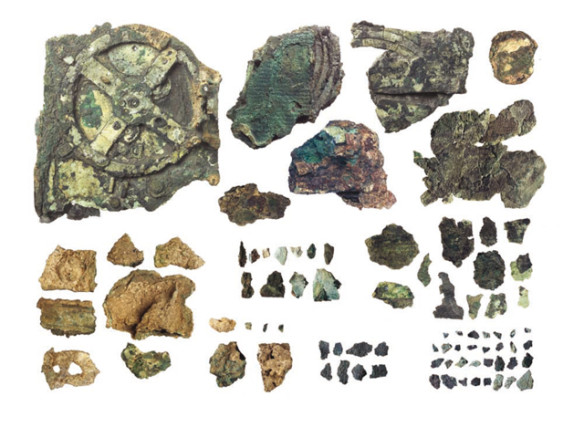
\includegraphics[height=2.1in]{machine-d-Anticythere-c.jpg}
  \end{center}

  \vfill
  \begin{center}
    \textit{Antikythera mechanism}
  \end{center}
\end{frame}

\begin{frame}
  \frametitle{Relational Database Management System}

  \begin{center}
    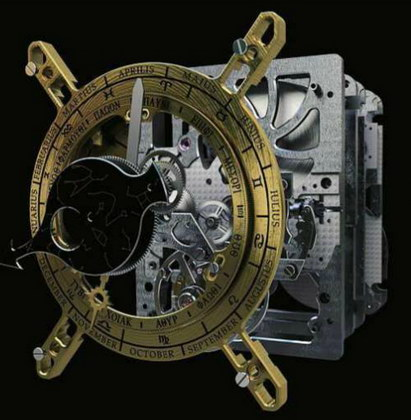
\includegraphics[height=2.1in]{anticy6.jpg}
  \end{center}

  \vfill
  \begin{center}
    \textit{Antikythera mechanism}
  \end{center}
\end{frame}

\begin{frame}
  \frametitle{Relational Database Management System}

  \begin{center}
    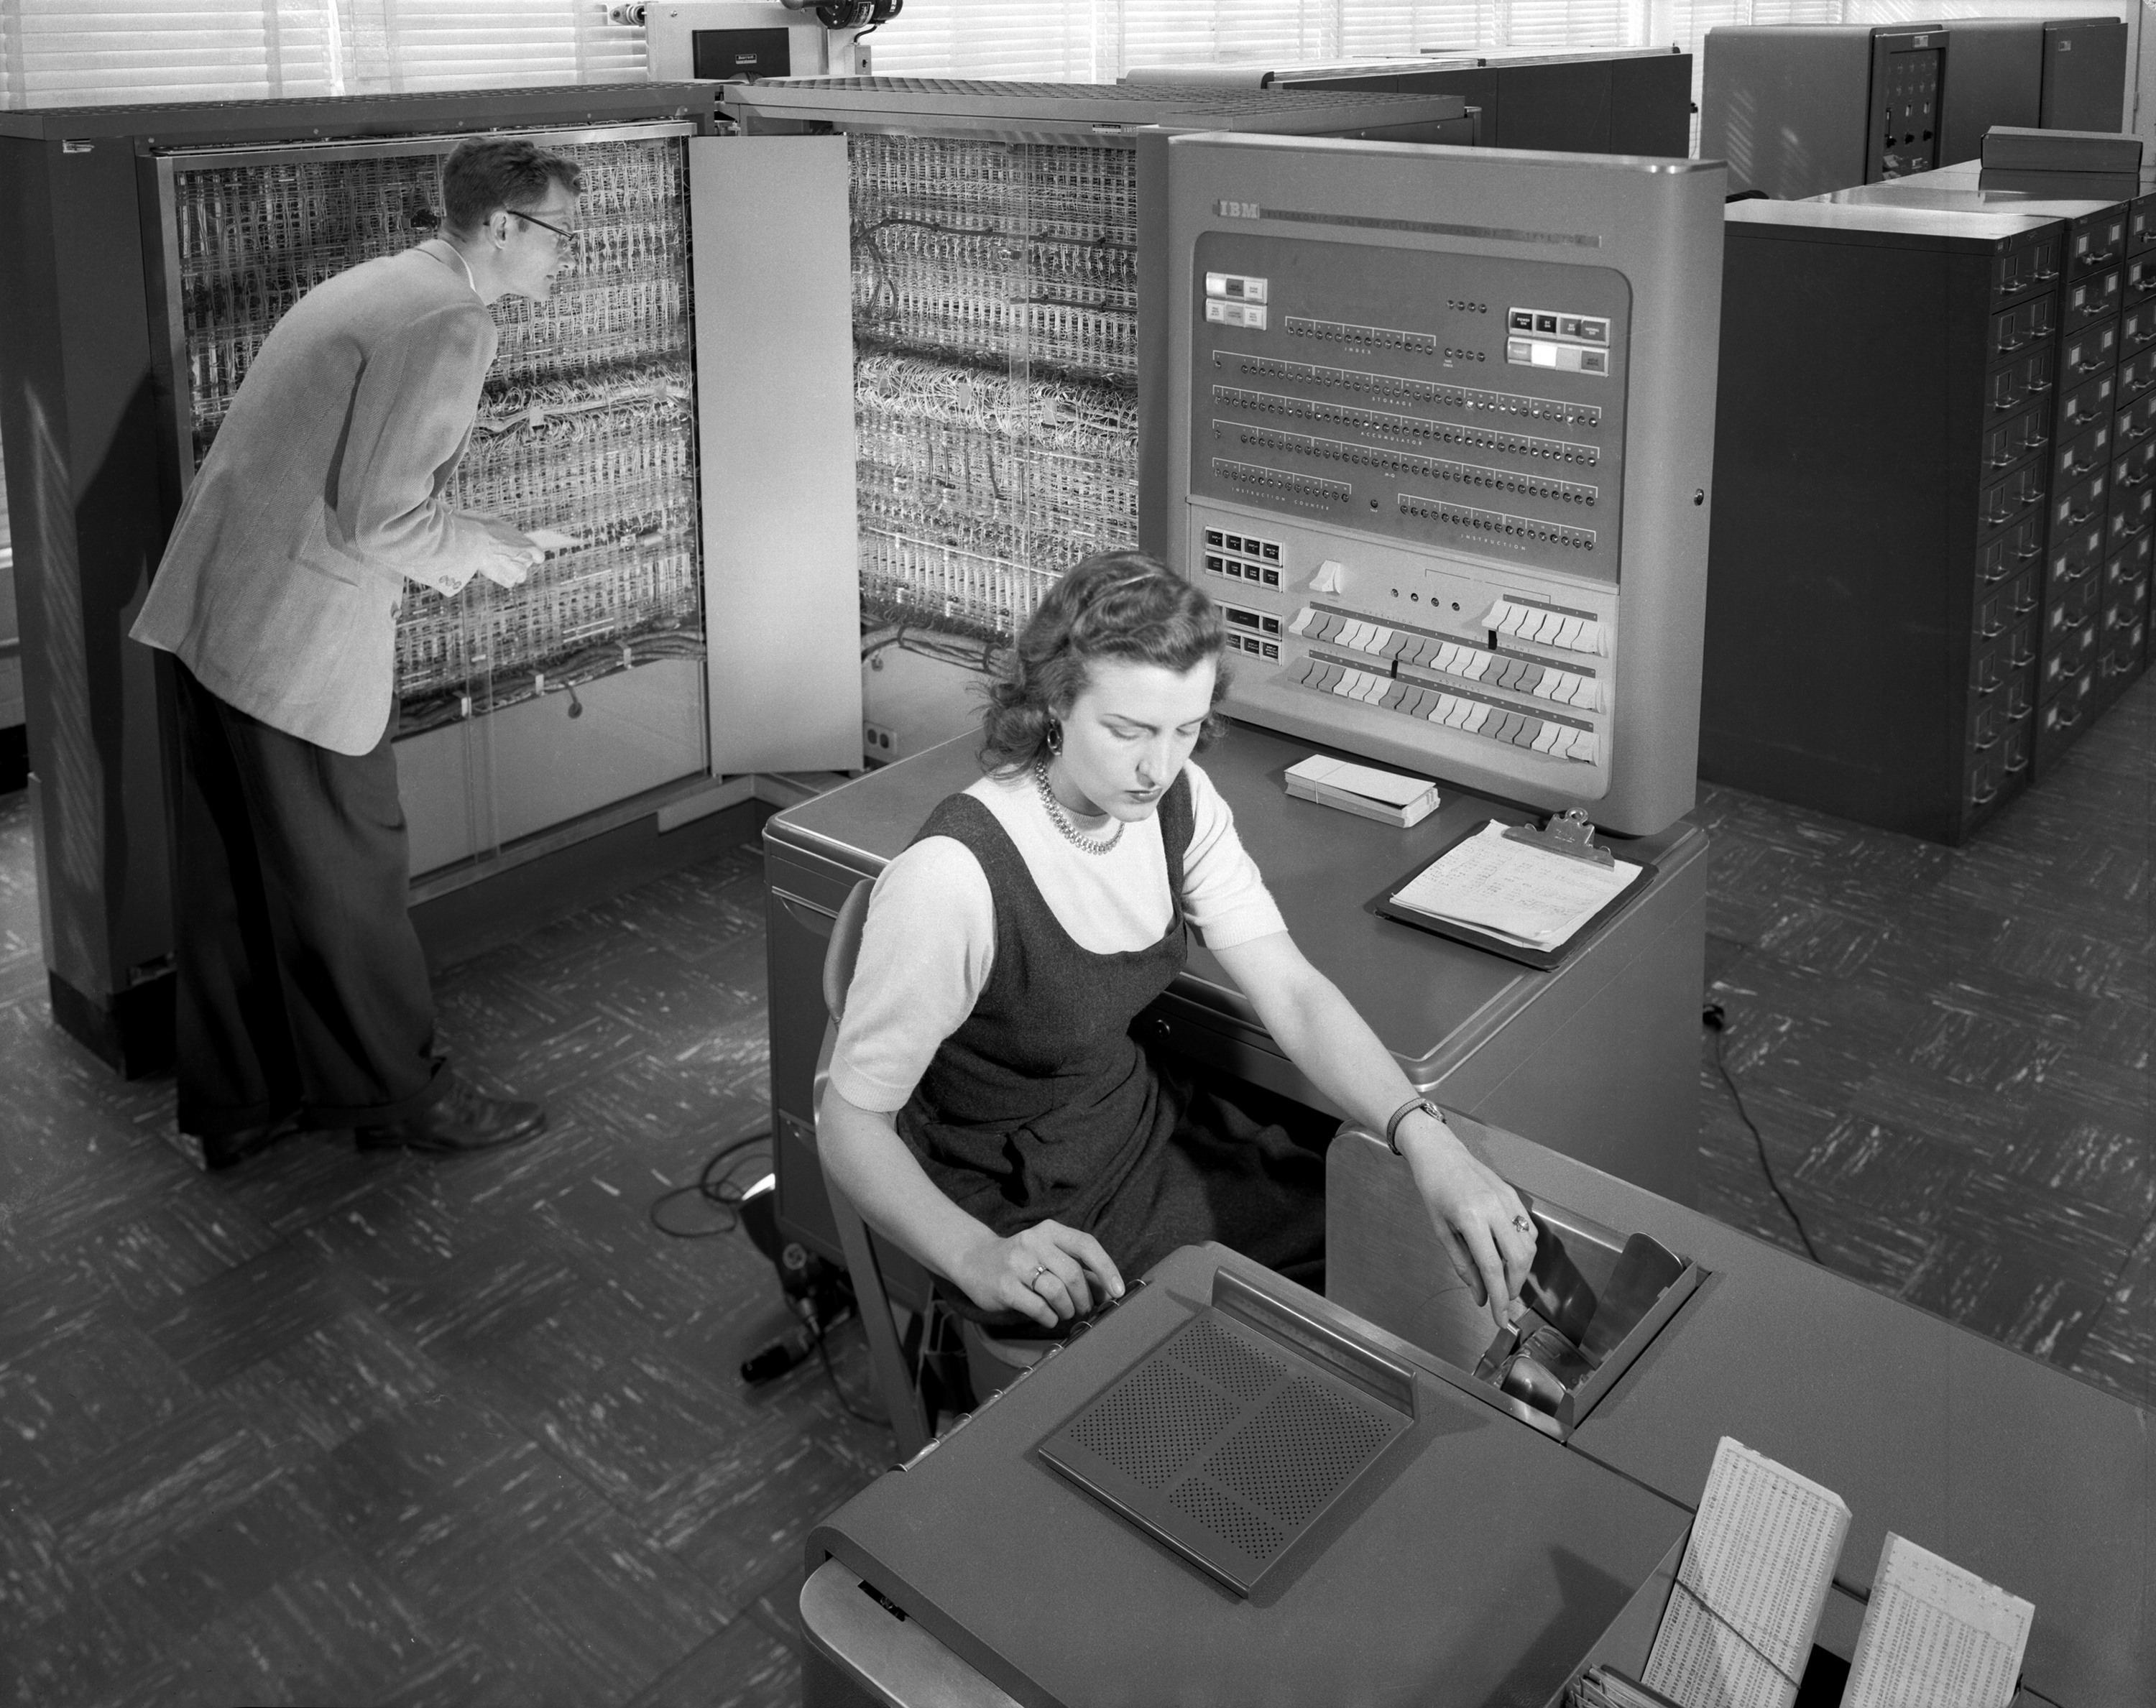
\includegraphics[height=2.1in]{IBM_Electronic_Data_Processing_Machine_-_GPN-2000-001881.jpg}
  \end{center}
\end{frame}

\begin{frame}
  \begin{center}
    \textsc{\Huge PostgreSQL is YeSQL!}
    \vfill

    
\includegraphics[height=9em]{postgres-logo.eps}
  \end{center}
\end{frame}

\begin{frame}
  \begin{center}
    \textsc{\Huge PostgreSQL is YeSQL!}
    \vfill

    
\includegraphics[height=9em]{nosql-bigdata.png}
  \end{center}
\end{frame}

\begin{frame}
  \frametitle{Relational Database Management System}

  \begin{columns}[c]
    \column{.5\textwidth} 
    \begin{center}
      
\includegraphics[height=9em]{caution_acid.png}
    \end{center}

    \column{.5\textwidth}
    \begin{center}
      
\includegraphics[height=12em]{sql.png}
    \end{center}
  \end{columns}
\end{frame}

\begin{frame}
  \frametitle{Relational Database Management System}

  \begin{center}
    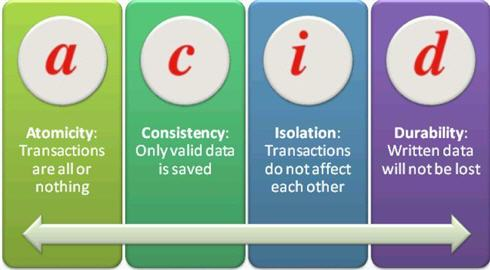
\includegraphics[height=2.1in]{acid-details.jpg}
  \end{center}
\end{frame}

\begin{frame}
  \frametitle{Relational Database Management System}

  \center{\Huge D is for Durability}
  
  \begin{center}
    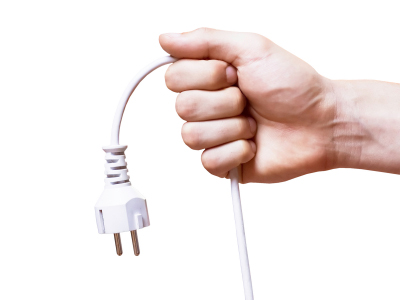
\includegraphics[height=2.1in]{cord-unplugged.jpg}
  \end{center}
\end{frame}

\begin{frame}
  \frametitle{Transactions}

  \center{\Huge A is for Atomic, that is, \textit{Transactions}}

  \begin{center}
    
\includegraphics[height=1.6in]{rollback-wordmark.png}
  \end{center}
\end{frame}

\begin{frame}[fragile]
  \frametitle{Transactions}

  \begin{minted}{postgresql}
    BEGIN;
      DROP TABLE critical_data;
    ROLLBACK;
  \end{minted}
\end{frame}

\begin{frame}
  \frametitle{Consistent Hot Backups}

  \center{\Huge I is for Isolated, that is, \textit{Transactions}}

  \begin{center}
    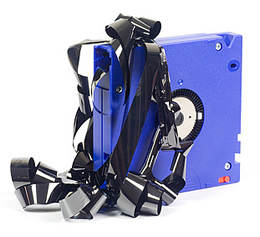
\includegraphics[height=2.1in]{online-backup.jpg}
  \end{center}
\end{frame}

\begin{frame}
  \frametitle{You don't want backups, you want data loss recovery!}

  \begin{center}
    
\includegraphics[height=2.1in]{Data-Recovery-Service-Icon.jpg}
  \end{center}
\end{frame}

\begin{frame}
  \frametitle{Consistency}

  \center{\Huge C is for Consistency}

  \begin{center}
    
\includegraphics[height=2.1in]{bits.jpeg}
  \end{center}
\end{frame}

\begin{frame}
  \frametitle{Scaling: up or out?}

  \begin{center}
    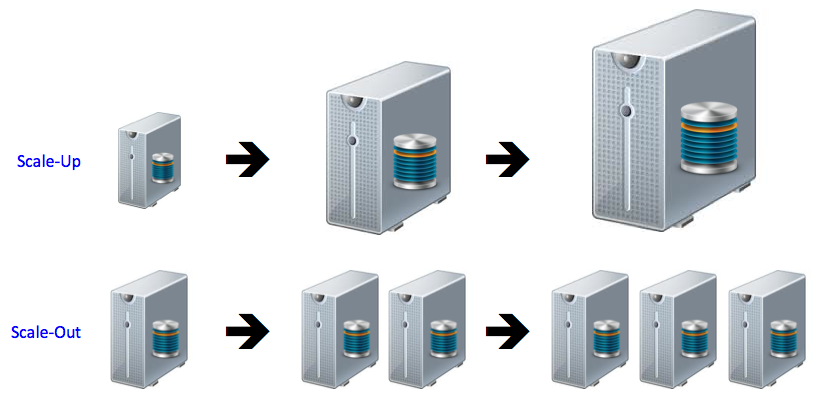
\includegraphics[height=2.1in]{KB_Scale_Out-Up.png}
  \end{center}
\end{frame}

\begin{frame}
  \frametitle{High Availability of Services and Data}

  \begin{center}
    
\includegraphics[height=2.1in]{distribution.jpg}
  \end{center}
\end{frame}

\begin{frame}[fragile]
  \frametitle{High Availability: Consistency and Durability}

  \begin{center}
    \begin{tikzpicture}[thick]
      \tikzstyle{node}=[minimum width=2.3cm,minimum height=1.3cm,
        rectangle,rounded corners=10pt,draw,
        fill=blue!20]

      \node[node]                 (P)  at (0,0)   {\Large Primary};
      \node[node][fill=orange!40] (A)  at (0,-3.2)  {\Large Archive};
      \node[node][fill=violet!20] (S1) at (-4,-5.2) {\Large Standby 1};
      \node[node][fill=violet!40] (S2) at (4,-5.2)  {\Large Standby 2};

      \tikzstyle{sr}=[->,dotted,very thick,>=latex]
      \tikzstyle{ar}=[->,>=latex]
      \tikzstyle{rc}=[->,dashed,>=latex]

      \draw[ar] (P) -- (A)
      node [midway,fill=white] {\texttt{archive\_command}};

      \draw[sr] (P) edge[bend right]
      node[pos=0.5,fill=white] {\textbf{Streaming Replication}}
      (S1);

      \draw[sr] (P) edge[bend left]
      node[pos=0.5,fill=white,text=violet]
      {\textbf{\textit{Streaming Replication}}}
      (S2);

      \draw[rc] (A) |- (S2)
      node [midway,fill=white,text=violet]
      {\texttt{restore\_command}};
    \end{tikzpicture}
  \end{center}
\end{frame}

\begin{frame}[fragile]
  \frametitle{High Availability}

  \begin{center}
    \begin{tikzpicture}[thick]
      \tikzstyle{node}=[minimum width=2cm,minimum height=1.5cm,
        rectangle,rounded corners=10pt,draw,
        fill=blue!20]

      \node[] (DC1)  at (-1,2.1)   {\Large \textbf{DC1}};
      \node[] (DC2)  at (1,2.1)    {\Large \textbf{DC2}};
      
      \node[node][fill=orange!40] (SR) at (-5,-3.5)  {\Large SR};
      \node[node][fill=violet!20] (S1) at (-2,-3.5)  {\Large S1};
      \node[node][fill=green!40]  (P1)  at (-2,0)  {\Large P1};

      \node[node][fill=green!40]  (P2) at  (2,0)   {\Large P2};
      \node[node][fill=violet!40] (S2) at (2,-3.5)   {\Large S2};
      \node[node][fill=violet!40] (S3) at (5,-3.5)   {\Large S3};

      \tikzstyle{bdr}=[<->,very thick,>=latex,double,double distance=1pt]
      \tikzstyle{sr}=[->,dotted,very thick,>=latex]
      \tikzstyle{ar}=[->,>=latex]
      \tikzstyle{rc}=[->,dashed,>=latex]

      \draw [dashed] (0,3) -- (0,-5);

      \draw[bdr] (P1) -- (P2) node [midway,text=violet,above]
           {\textbf{\textit{\Large BDR}}};
           
           \draw[sr] (P1) to[out=-135,in=90] node [midway] {} (SR);
           \draw[sr] (P1) -- (S1) node[pos=0.5] {};

           \draw[sr] (P2) -- (S2) node [midway] {};
           \draw[sr] (P2) to[out=-45,in=90] node [midway] {} (S3);

    \end{tikzpicture}
  \end{center}
\end{frame}

\begin{frame}
  \frametitle{Consistency}

  \begin{center}
    
\includegraphics[height=2.1in]{bits.jpeg}
  \end{center}
\end{frame}

\begin{frame}[fragile]
  \frametitle{Data Types and Constraints}

  \center{Data integrity First Layer: data type}
  \vfill
  
  \begin{columns}[c]

    \column{.5\textwidth} 
    \begin{itemize}
    \item \texttt{Integer}
    \item \texttt{Arbitrary precision numbers, UUID}
    \item \texttt{Floating point}
    \item \texttt{Character, Text}
    \item \texttt{Bytea, bitstring}
    \item \texttt{Date/Time, Time Zones}
    \end{itemize}  

    \column{.5\textwidth}
    \begin{itemize}
    \item \texttt{Boolean}
    \item \texttt{Enum, Arrays, Composite Types, Range Types}
    \item \texttt{Point, Line Segments, Boxes}
    \item \texttt{Paths, Polygons, Circles}
    \item \texttt{Inet, CIDR, Macaddr}
    \item \texttt{JSON, XML}
    \end{itemize}

  \end{columns}
\end{frame}


\begin{frame}[fragile]
  \frametitle{Advanced data types and constraints}

\begin{columns}
\column{.5\textwidth}
  \begin{minted}{postgresql}
 CREATE TABLE reservation
 (
   room      text,
   professor text,
   during    period,
   EXCLUDE USING gist
   (
       room with =,
     during with &&
   )
  );
  \end{minted}
  \column{.5\textwidth}
  \begin{minted}{postgresql}
  CREATE TABLE circles (
    c circle,
    EXCLUDE USING gist
      (c WITH &&)
  );
  \end{minted}
\end{columns}
\end{frame}

\begin{frame}
  \frametitle{\textsc{Structured Query Language}}

  \begin{center}
    
\includegraphics[height=2.1in]{sql.png}
  \end{center}
\end{frame}


\begin{frame}[fragile]
  \frametitle{Finding the last counter value before \textit{reset}}

\begin{columns}
\column{.65\textwidth}
\center{\textit{Write some \alert{SQL} here}}
\column{.35\textwidth}
\begin{minted}{postgresql}
 tick | nb | max 
------+----+-----
    1 |  0 |    
    2 | 10 |    
    3 | 20 |    
    4 | 30 |    
    5 | 40 |  40
    6 |  0 |    
    7 | 20 |    
    8 | 30 |    
    9 | 60 |  60
(9 rows)
\end{minted}
\end{columns}
\end{frame}

\begin{frame}[fragile]
  \frametitle{Window Functions: \texttt{lead() over()}}

\begin{columns}
\column{.65\textwidth}
\begin{minted}{postgresql}
  select tick,
         nb,
         lead(nb) over (order by tick)
    from measures;
\end{minted}

\column{.35\textwidth}
\begin{minted}{postgresql}
 tick | nb | lead 
------+----+------
    1 |  0 |   10
    2 | 10 |   20
    3 | 20 |   30
    4 | 30 |   40
    5 | 40 |    0
    6 |  0 |   20
    7 | 20 |   30
    8 | 30 |   60
    9 | 60 |     
(9 rows)
\end{minted}
\end{columns}
\end{frame}

\begin{frame}[fragile]
  \frametitle{Window Functions and \texttt{CASE}}

\begin{columns}
\column{.65\textwidth}
\begin{minted}{postgresql}
  select tick, nb,
         case when lead(nb) over w < nb
              then nb

              when lead(nb) over w is null
              then nb

              else null
          end as max
    from measures
  window w as (order by tick);
\end{minted}
\column{.35\textwidth}
\begin{minted}{postgresql}
 tick | nb | max 
------+----+-----
    1 |  0 |    
    2 | 10 |    
    3 | 20 |    
    4 | 30 |    
    5 | 40 |  40
    6 |  0 |    
    7 | 20 |    
    8 | 30 |    
    9 | 60 |  60
(9 rows)
\end{minted}
\end{columns}
\end{frame}

\begin{frame}[fragile]
  \frametitle{PostgreSQL Extensibility}

  \center{PostgreSQL is \textit{highly} \textbf{extensible}}
  \vfill

\begin{center}
  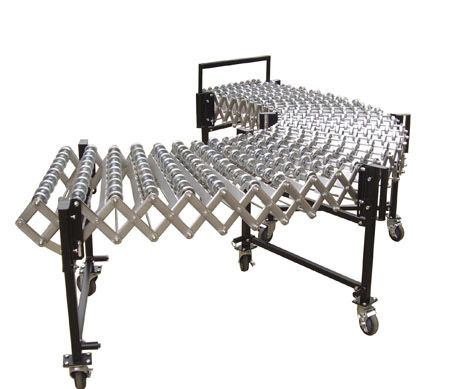
\includegraphics[height=15em]{extensible.jpg}
\end{center}
\end{frame}

\begin{frame}[fragile]
  \frametitle{B-Tree}

  \center{\textit{Balanced Tree}, the default index type}
  \vfill

\begin{columns}[c]
\column{.55\textwidth} 

  \begin{itemize}
  \item Built for speed
  \item \textit{unique} concurrency tricks
  \item Balanced
  \item support function: \texttt{cmp}
  \item operators: \texttt{<= < = > >=}
  \end{itemize}

\column{.45\textwidth}
\begin{center}
  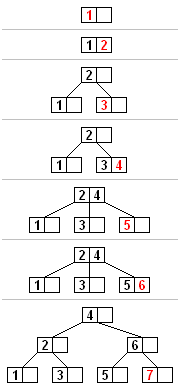
\includegraphics[height=14em]{B_tree_insertion_example.png}
\end{center}
\end{columns}
\end{frame}


\begin{frame}[fragile]
  \frametitle{Generalized Index Search Tree}

  \center{GiST or the Indexing API}
  \vfill

\begin{columns}[c]
\column{.55\textwidth} 

  \begin{itemize}
  \item Built for comfort
  \item Balanced
  \item API: \texttt{consistent}, \texttt{same}, \texttt{union}
  \item API: \texttt{penalty}, \texttt{picksplit}
  \item API: \texttt{compress}, \texttt{decompress}
  \item operators: \texttt{@> <@ \&\& @@ = \&< \&> <<| ...}
  \end{itemize}

\column{.45\textwidth}
\begin{center}
  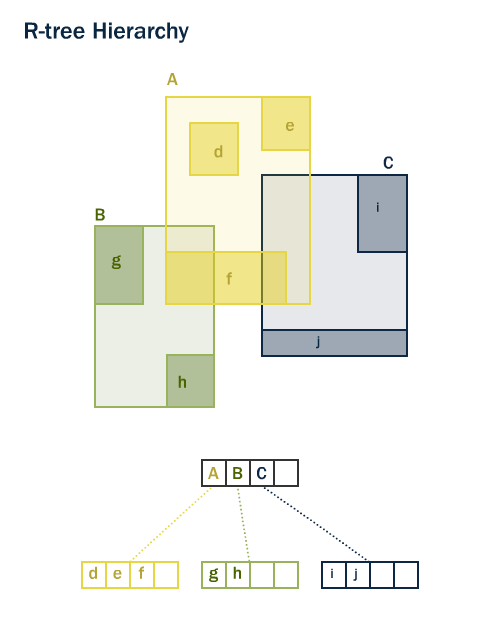
\includegraphics[height=14em]{rtree.png}
\end{center}
\end{columns}
\end{frame}


\begin{frame}[fragile]
  \frametitle{Generalized Inverted iNdex}

  \center{Indexing several pointers per value, inversed cardinality}
  \vfill

\begin{columns}[c]
\column{.55\textwidth} 

  \begin{itemize}
  \item Built for Text Search and Arrays
  \item Balanced
  \item API: \texttt{compare}, \texttt{consistent}
  \item API: \texttt{extractValue}, \texttt{extractQuery}
  \item operators: \texttt{@> <@ \&\& =}
  \end{itemize}

\column{.45\textwidth}
\begin{center}
  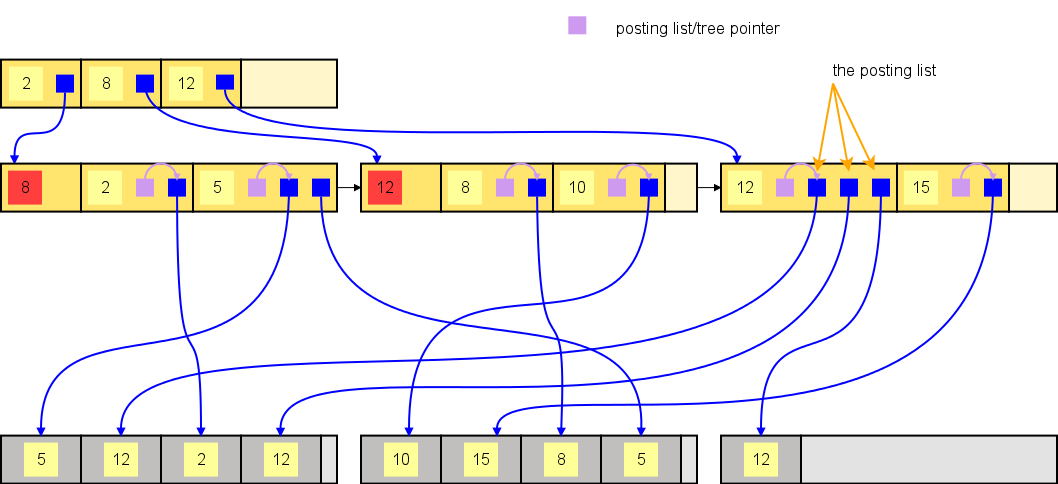
\includegraphics[height=5em]{gin.png}
\end{center}
\end{columns}
\end{frame}

\begin{frame}[fragile]
  \frametitle{GIN indexes main use case}

  \center{\Huge PostgreSQL Full Text Search}
  \vfill

  \begin{center}
    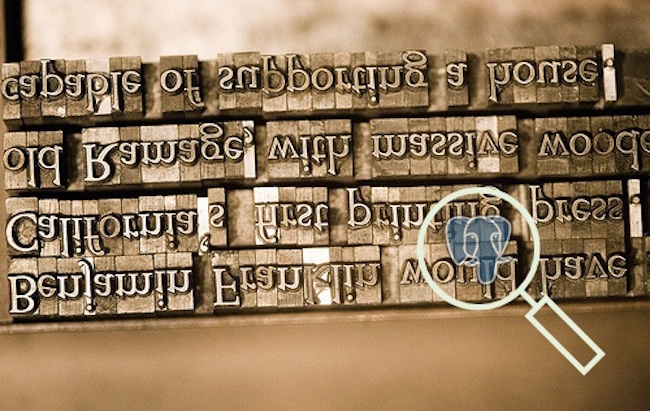
\includegraphics[height=15em]{pg_doc_search.jpg}
  \end{center}
\end{frame}

\begin{frame}[fragile]
  \frametitle{Spaced Partition GiST}

  \center{Unbalanced index, used for \Huge GIS}
  \vfill

  \begin{center}
    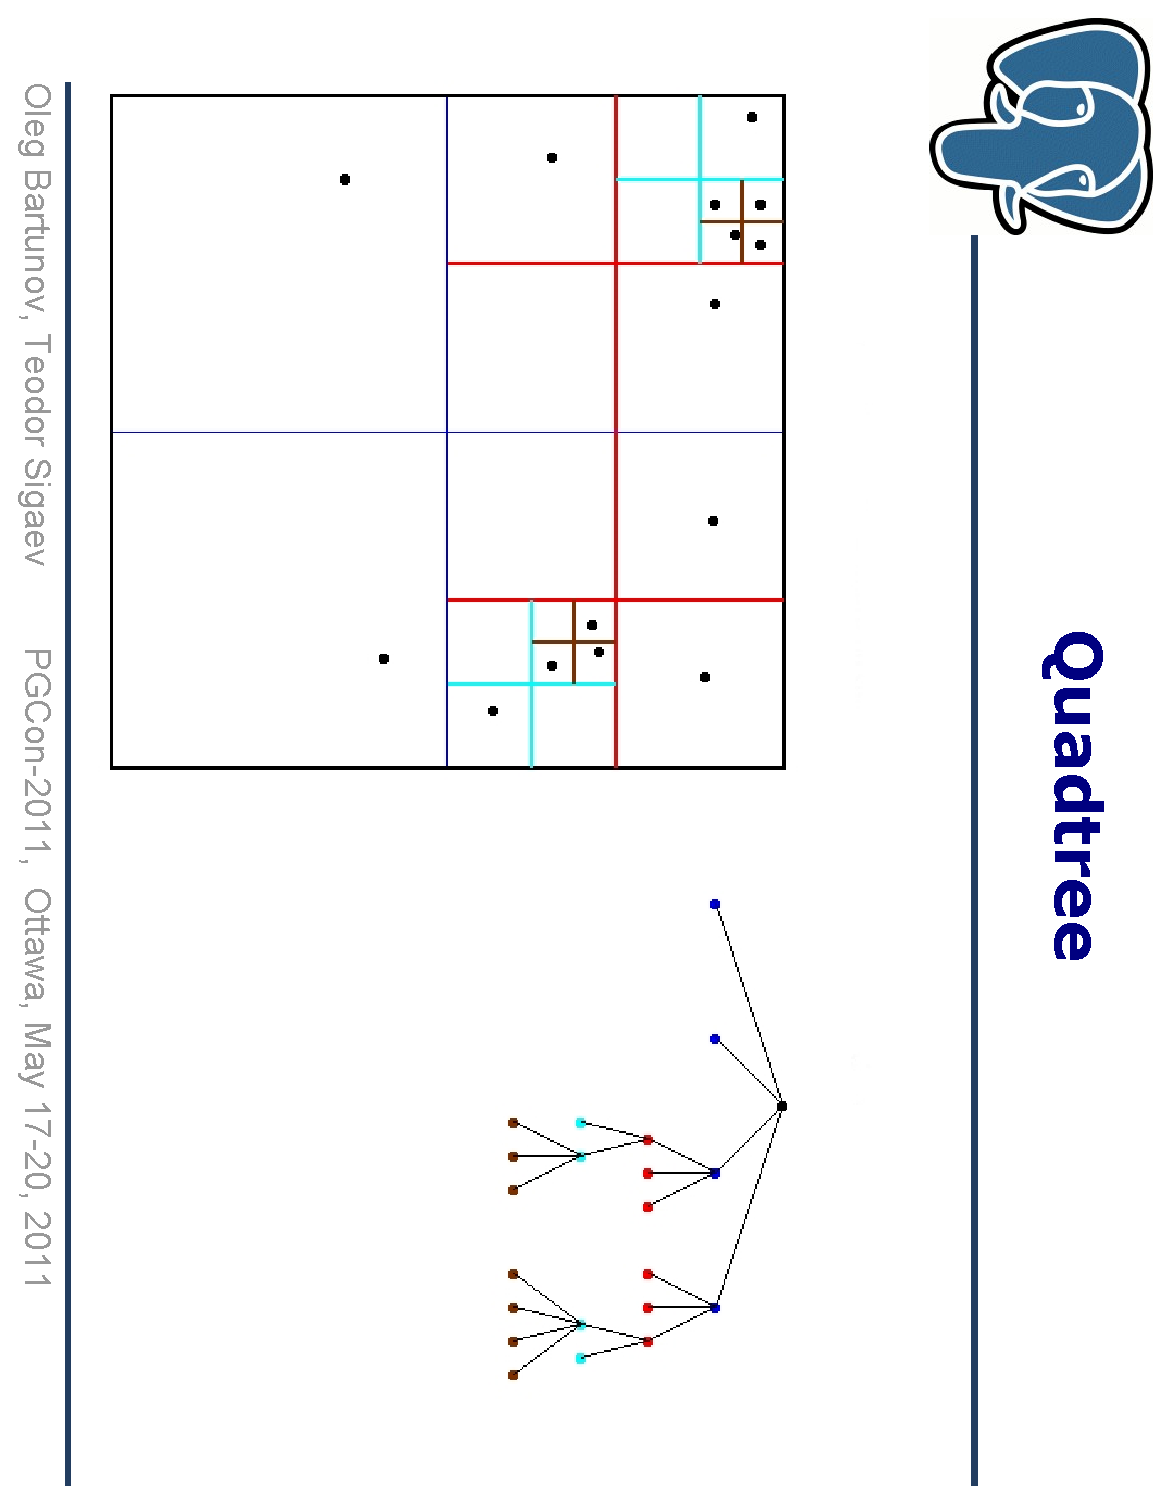
\includegraphics[height=15em]{sp-gist.eps}
  \end{center}
\end{frame}

\begin{frame}[fragile]
  \frametitle{BRIN}

  \center{Block Range Index for Big Data}
  \vfill
  
  \begin{center}
    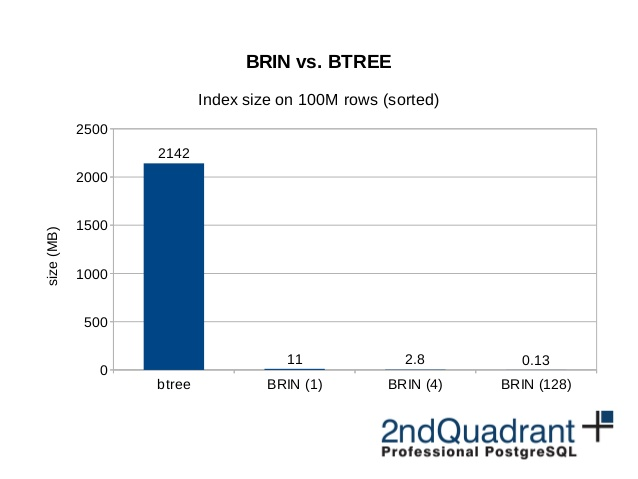
\includegraphics[height=15em]{brin.jpg}
  \end{center}
\end{frame}

\begin{frame}
  \frametitle{\textsc{Structured Query Language}}

  \begin{center}
    
\includegraphics[height=2.1in]{sql.png}
  \end{center}
\end{frame}

\begin{frame}[fragile]
  \frametitle{IP Ranges, \texttt{ip4r}, Geolocation}

  \center{PostgreSQL allows using SQL and JOINs to match IP4R with geolocation.}
  \vfill

\begin{columns}
\column{.45\textwidth}
\begin{minted}{postgresql}
 select *
   from geolite.blocks
   join geolite.location
        using(locid)
  where iprange
            >>=
        '74.125.195.147';
\end{minted}
\column{.55\textwidth}
\begin{center}
  
\includegraphics[height=9em]{geolocation-clic.png}
\end{center}
\end{columns}
\end{frame}

\begin{frame}[fragile]
  \frametitle{IP Ranges, \texttt{ip4r}, Geolocation}

  \center{PostgreSQL allows using SQL and JOINs to match IP4R with geolocation.}
  \vfill

\begin{columns}
\column{.45\textwidth}
\begin{minted}{postgresql}
 select *
   from geolite.blocks
   join geolite.location
        using(locid)
  where iprange
            >>=
        '74.125.195.147';
\end{minted}
\column{.55\textwidth}
\begin{minted}{postgresql}
-[ RECORD 1 ]----------------------------
locid      | 2703
iprange    | 74.125.189.24-74.125.255.255
country    | US
region     | CA
city       | Mountain View
postalcode | 94043
location   | (-122.0574,37.4192)
metrocode  | 807
areacode   | 650

Time: 1.335 ms
\end{minted}
\end{columns}
\end{frame}

\begin{frame}[fragile]
  \frametitle{Geolocation: \texttt{ip4r} meets \text{earthdistance}}

\begin{center}
  
\includegraphics[height=12em]{geolocation.png}
\end{center}
\end{frame}

\begin{frame}[fragile]
  \frametitle{Some pubs nearby... some place...}

\begin{columns}
\column{.5\textwidth}
\begin{minted}{postgresql}
with geoloc as
 (
  select location as l
    from location
    join blocks using(locid)
   where iprange
         >>=
         '212.58.251.195'
 )
  select name,
         pos <@> l miles
    from pubnames, geoloc
order by pos <-> l
   limit 10;
\end{minted}  
\column{.5\textwidth}
\begin{minted}{postgresql}
        name        | miles 
--------------------+-------
 Blue Anchor        | 0.299
 Dukes Head         | 0.360
 Blue Ball          | 0.337
 Bell (aka The Rat) | 0.481
 on the Green       | 0.602
 Fox & Hounds       | 0.549
 Chequers           | 0.712
 Sportsman          | 1.377
 Kingswood Arms     | 1.205
 Tattenham Corner   | 2.007
(10 rows)

Time: 3.275 ms
\end{minted}  
\end{columns}
\end{frame}

\begin{frame}
  \frametitle{NBA Games Statistics}

  \begin{center}
    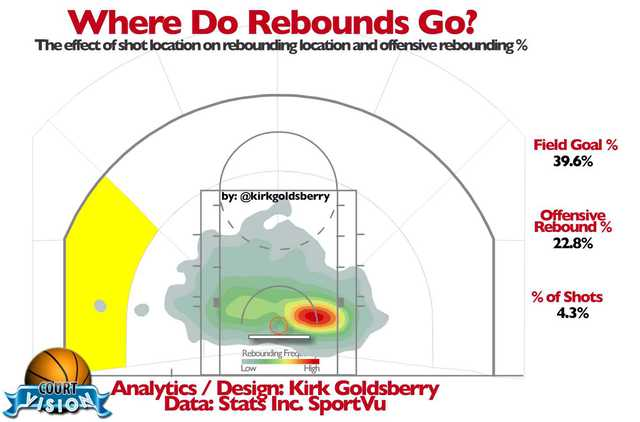
\includegraphics[height=2.1in]{reboundsc1.jpg}
  \end{center}
\end{frame}

\begin{frame}
  \frametitle{NBA Games Statistics}

  An interesting factoid: the team that recorded the fewest defensive
  rebounds in a win was the 1995-96 Toronto Raptors, who beat the Milwaukee
  Bucks 93-87 on 12/26/1995 despite recording only 14 defensive rebounds.
\end{frame}

\begin{frame}[fragile]
  \frametitle{PostgreSQL Data Mining}

\begin{minted}{postgresql}
with stats(game, team, drb, min) as (
    select ts.game, ts.team, drb, min(drb) over ()
      from team_stats ts
           join winners w on w.id = ts.game
                         and w.winner = ts.team
)
select game.date::date,
       host.name || ' -- ' || host_score as host,
       guest.name || ' -- ' || guest_score as guest,
       stats.drb as winner_drb
  from stats
       join game on game.id = stats.game
       join team host on host.id = game.host
       join team guest on guest.id = game.guest
 where drb = min;
\end{minted}
\end{frame}

\begin{frame}[fragile]
  \frametitle{PostgreSQL Data Mining}

\begin{minted}[fontsize=\footnotesize]{postgresql}
-[ RECORD 1 ]----------------------------
date       | 1995-12-26
host       | Toronto Raptors -- 93
guest      | Milwaukee Bucks -- 87
winner_drb | 14
-[ RECORD 2 ]----------------------------
date       | 1996-02-02
host       | Golden State Warriors -- 114
guest      | Toronto Raptors -- 111
winner_drb | 14
-[ RECORD 3 ]----------------------------
date       | 1998-03-31
host       | Vancouver Grizzlies -- 101
guest      | Dallas Mavericks -- 104
winner_drb | 14
-[ RECORD 4 ]----------------------------
date       | 2009-01-14
host       | New York Knicks -- 128
guest      | Washington Wizards -- 122
winner_drb | 14

Time: 126.276 ms
\end{minted}
\end{frame}

\begin{frame}
  \frametitle{Pure SQL Histogram drawing}

  \begin{center}
    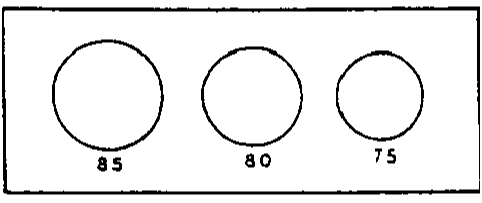
\includegraphics[height=1.8in]{histogram.png}
  \end{center}
\end{frame}

\begin{frame}[fragile]
  \frametitle{Pure SQL Histogram drawing}
  
  \begin{minted}{postgresql}
with drb_stats as (
    select min(drb) as min,
           max(drb) as max
      from team_stats
),
     histogram as (
   select width_bucket(drb, min, max, 9) as bucket,
          int4range(min(drb), max(drb), '[]') as range,
          count(*) as freq
     from team_stats, drb_stats
 group by bucket
 order by bucket
)
 select bucket, range, freq,
        repeat('*', (freq::float / max(freq) over() * 30)::int) as bar
   from histogram;
  \end{minted}
\end{frame}

\begin{frame}[fragile]
  \frametitle{Pure SQL Histogram drawing}
  
  \begin{minted}{postgresql}
 bucket |  range  | freq  |              bar               
--------+---------+-------+--------------------------------
      1 | [10,15) |    52 | 
      2 | [15,20) |  1363 | **
      3 | [20,25) |  8832 | *************
      4 | [25,30) | 20917 | ******************************
      5 | [30,35) | 20681 | ******************************
      6 | [35,40) |  9166 | *************
      7 | [40,45) |  2093 | ***
      8 | [45,50) |   247 | 
      9 | [50,54) |    20 | 
     10 | [54,55) |     1 | 
(10 rows)

Time: 53.570 ms
\end{minted}
\end{frame}

\begin{frame}[fragile]
  \frametitle{Writeable \texttt{CTE}}
  
  \begin{minted}{postgresql}
with queue as (
   insert into queue (extension)
        select id
          from extension
         where shortname = $1
  returning id, extension
)
select q.id, e.id as ext_id,
       e.fullname, e.uri, e.description
  from      queue q
       join extension e on q.extension = e.id;    
  \end{minted}
\end{frame}

\begin{frame}
  \frametitle{PostgreSQL Joins}

  \begin{center}
    
\includegraphics[height=12em]{huge-full-outer-join.jpg}
  \end{center}
\end{frame}

\begin{frame}[fragile]
  \frametitle{PostgreSQL Joins}

  \begin{minted}{postgresql}
WITH upd AS (
    UPDATE target t
       SET counter = t.counter + s.counter,
      FROM source s
     WHERE t.id = s.id
 RETURNING s.id
)
INSERT INTO target(id, counter)
     SELECT id, sum(counter)
       FROM source s LEFT JOIN upd t USING(id)
      WHERE t.id IS NULL
   GROUP BY s.id
   RETURNING t.id
  \end{minted}
\end{frame}

\begin{frame}[fragile]
  \frametitle{PostgreSQL Lateral Joins}

  \center{Fetch the 10 most recent news for each topic (\textbf{Top-N})}
  \vfill
  
  \begin{minted}{postgresql}
SELECT n.*
  FROM subscriptions s
  JOIN LATERAL (SELECT *
                  FROM news n
                 WHERE n.topic = s.topic
                 ORDER BY n.created DESC
                 LIMIT 10
               ) top_news ON (true)
 WHERE s.user_id = ?
 ORDER BY n.created DESC
 LIMIT 10
  \end{minted}
\end{frame}
 
\begin{frame}
  \begin{center}
    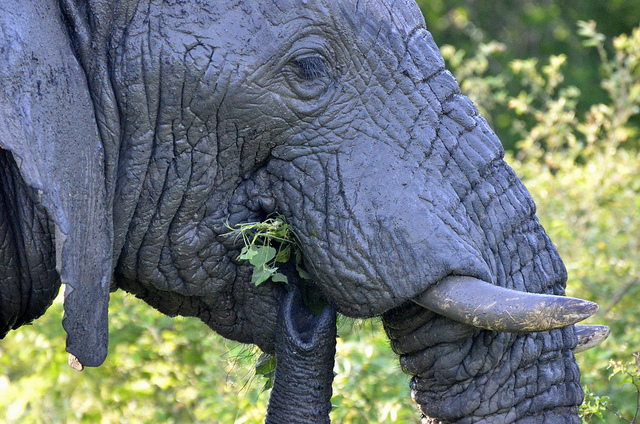
\includegraphics[height=21em]{postgresql-mongodb.jpg}
  \end{center}
\end{frame}

\begin{frame}
  \begin{center}
    \textsc{\Huge PostgreSQL is YeSQL!}
    \vfill

    
\includegraphics[height=9em]{postgres-logo.eps}
  \end{center}
\end{frame}

\begin{frame}
  \frametitle{Questions?}

  \begin{center}
    Now is the time to ask!
    \vfill

    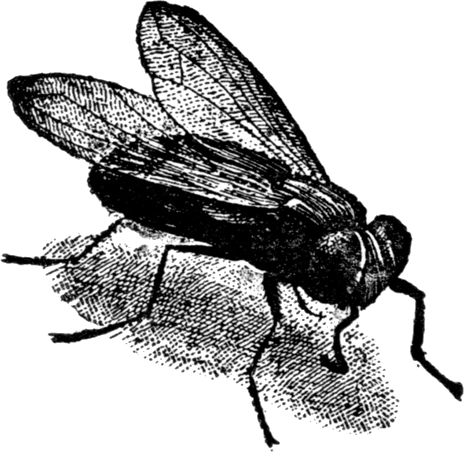
\includegraphics[height=9em]{fly.png}
  \end{center}
\end{frame}

\end{document}
